\documentclass[14pt,aspectratio=169]{beamer}
\usepackage[utf8]{inputenc}
\usepackage[spanish]{babel}
\usepackage{xcolor}
\usepackage{biblatex}
\addbibresource{presentacion.bib}
\setbeamertemplate{bibliography item}{\insertbiblabel}
\usepackage[autostyle=true]{csquotes}

\usetheme{Copenhagen}
%\setbeamercolor{background canvas}{bg=white}
\definecolor{verde}{rgb}{.25,.5,.25}
\usecolortheme[named=verde]{structure}

\usepackage{helvet}

\title{Edición ramificada}
\subtitle{la edición por venir}
\author{Alberto Moyano}
\date{22 de abril de 2024}
\institute{\url{https://github.com/albertomoyano/CHARLAUBA2}}

\setbeamertemplate{headline}{}
\setbeamertemplate{navigation symbols}{}
\setbeamercovered{transparent}

\begin{document}

	\begin{frame}
		\titlepage
	\end{frame}

\begin{frame}{Un solo origen}
	¿Qué es la edición ramificada en el campo editorial?\vspace{14pt}

	\begin{quote}
	Refiere a un modelo de producción a partir de un único origen, en donde se configuran salidas independientes para diferentes necesidades o requisitos sin afectar al origen principal.
	\end{quote}
\end{frame}

\begin{frame}{Modelo estrella}
	\begin{figure}
		\centering
		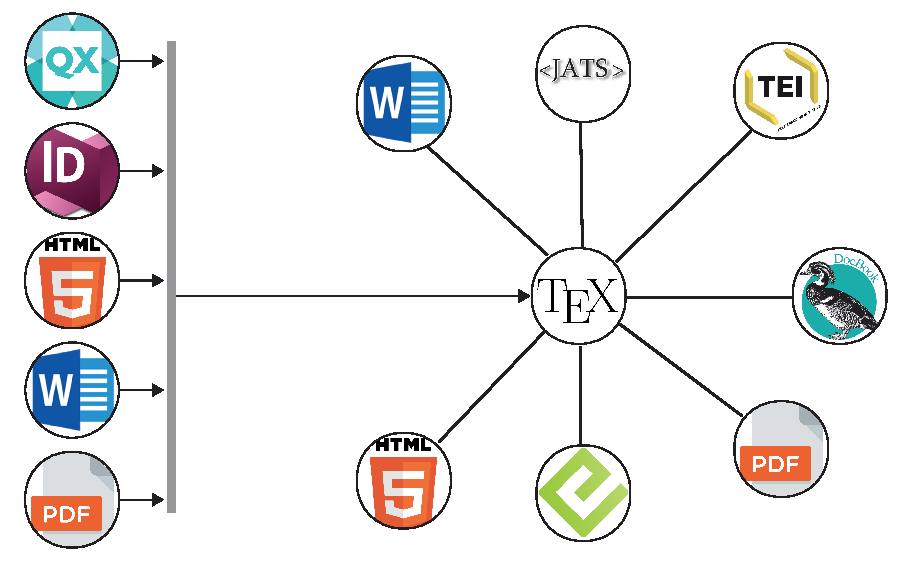
\includegraphics[width=.7\textwidth]{estrella.pdf}
	\end{figure}
\end{frame}

\begin{frame}{Modelo árbol}
	\begin{figure}
		\centering
		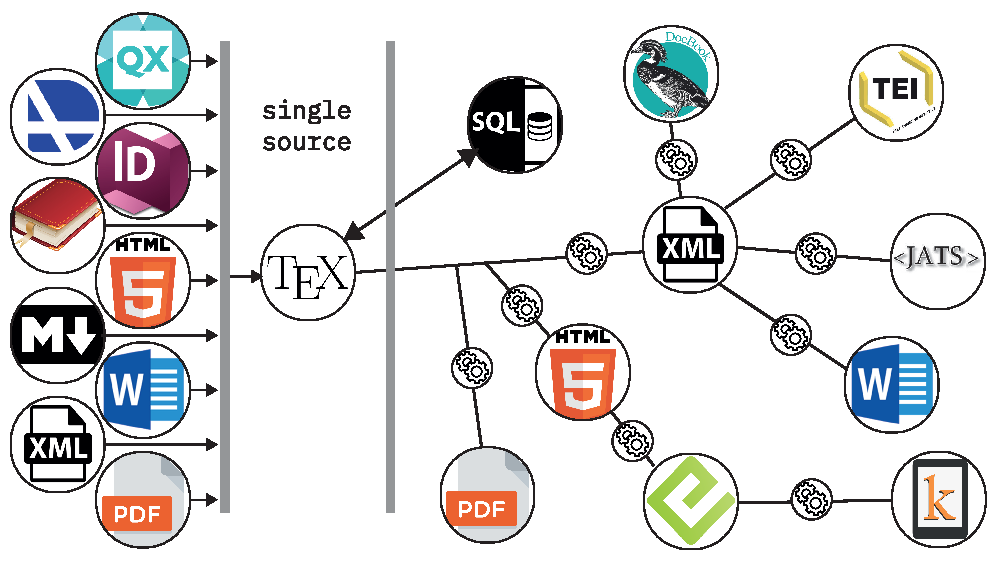
\includegraphics[width=.8\textwidth]{arbol.pdf}
	\end{figure}
\end{frame}

%\begin{frame}{Lenguajes de marcas}
%	\begin{enumerate}
%	\item Markdown: marcado ligero diseñado para ser fácil de leer y escribir, con una sintaxis básica.\\
%	\url{https://daringfireball.net/projects/markdown/}
%	\item AsciiDoc: marcado diseñado para ser fácil de leer y escribir, con una sintaxis simple y legible.\\
%	\url{https://asciidoc.org/}
%	\item LaTeX: sistema de preparación de documentos, se utiliza para la creación de documentos científicos.\\
%	\url{https://www.latex-project.org/}
%	\end{enumerate}
%\end{frame}

\begin{frame}{Algunas ventajas}
El modelo permite avanzar en un sistema de producción editorial flexible y multisoporte, Se pueden observar:

\begin{itemize}
	\item<2-> Capacidad para trabajo en modo colaborativo a través de ramas.
	\item<3-> Asegura la longevidad del contenido.
	\item<4-> No tiene dependencias binarias.
	\item<5-> En su mayoría las aplicaciones involucradas, poseen licencia MIT, BSD y GPL.
\end{itemize}
\end{frame}

\begin{frame}{Trabajando con gbTeXpublisher}
	\begin{figure}
		\centering
		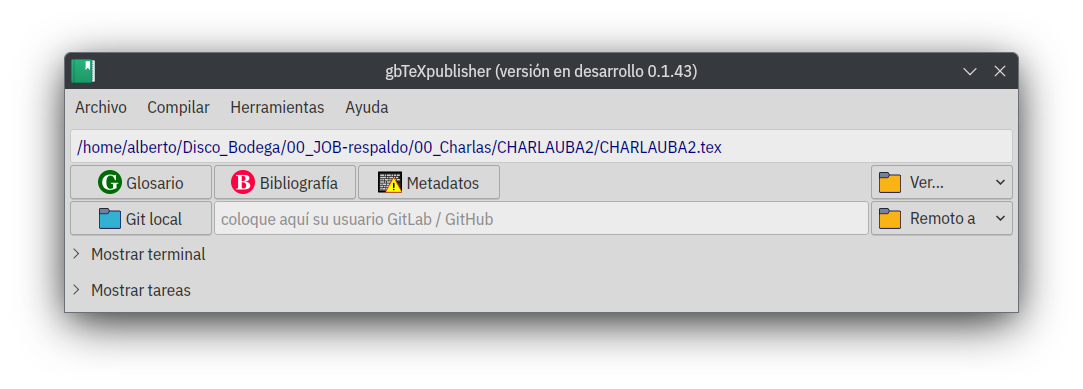
\includegraphics[width=.8\textwidth]{captura.png}
	\end{figure}
\end{frame}

%\nocite{*}
%\begin{frame}{Para saber más}
%	\printbibliography
%\end{frame}

\end{document}
